\chapter{Available Functionality and How to Use It}
\label{ch:modules}
% ##################################################################################################################

\hfill \textbf{Authors:} Andreas Horni, Kai Nagel

\begin{center} 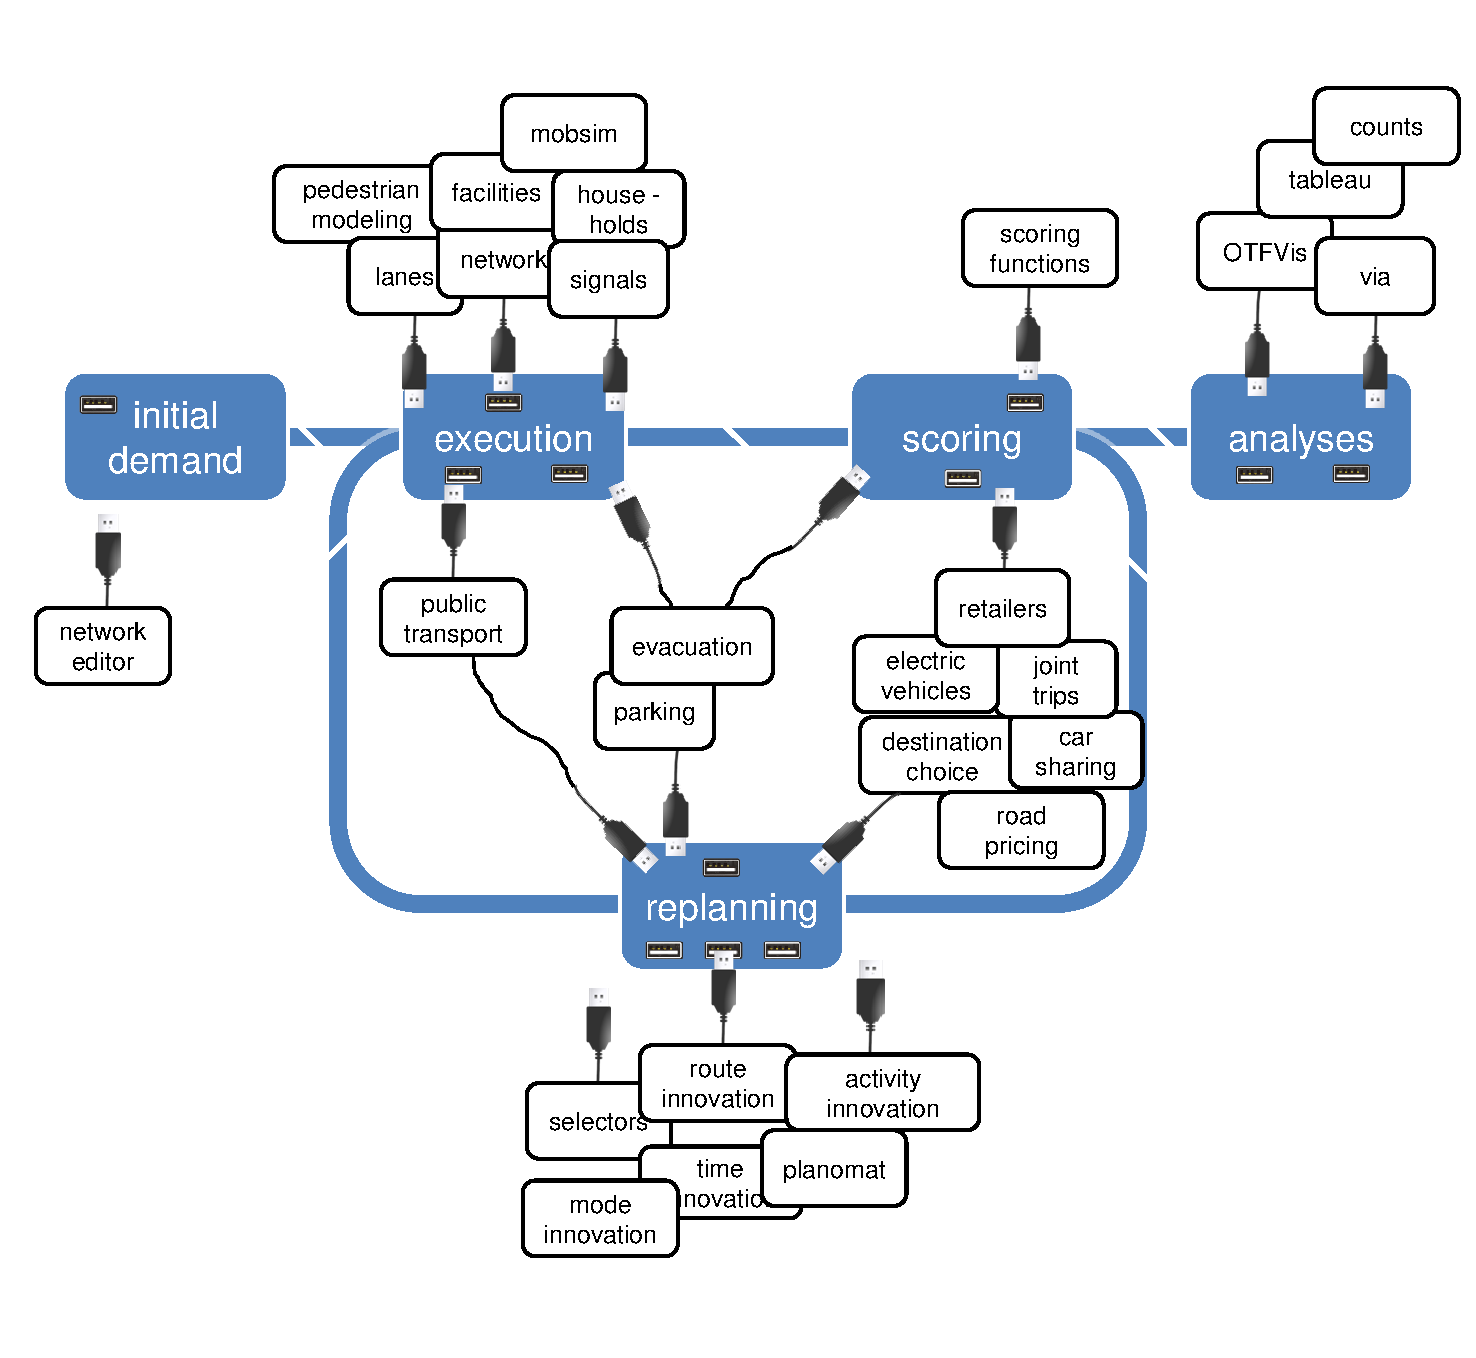
\includegraphics[width=0.5\textwidth, angle=0]{extending/figures/modules.pdf} \end{center}

%%%%%%%%%%%%%%%%%%%%%%%%%%%%%%%%%%%%%%%%%%%%
%%%%%%%%%%%%%%%%%%%%%%%%%%%%%%%%%%%%%%%%%%%%
\kai{need to clarify the factory concept somewhere (in the future probably just PopulationUtils.createActivity(...)).}

\ah{Section~\ref{sec:writing-scripts-java}}

\ah{added ``events'' container under ``Global Modules and Global Aspects''}

%%%%%%%%%%%%%%%%%%%%%%%%%%%%%%%%%%%%%%%%%%%%
%%%%%%%%%%%%%%%%%%%%%%%%%%%%%%%%%%%%%%%%%%%%

% ##################################################################################################################
In this chapter you will learn about the possibilities to extend, and customize \gls{matsim} by provided functionality. 
In Chapter~\ref{ch:extensionpoints} you will see how you can hook your own extensions into \gls{matsim}.

%%\kai{Frage mich im Moment, ob wir diejenigen ``Module'', die man per config aufrufen kann, nicht doch lieber bereits unter ``using'' beschreiben sollten.  Aber vielleicht ist das inzwischen fast egal, und wir sollten lieber Standard-MATSim komplett separat von jeder Art Variation halten.  ???}
%\ah{see Chapter~\ref{ch:configuring}}

% ##################################################################################################################
\section{MATSim Modularity}
\label{sec:matsim-modularity}

%% \kai{Andreas, haben wir noch eine Chance, diese Ungleichheiten in der Nomenklatur geradezuziehen?  
%% %contrib vs extension \url{https://matsim.atlassian.net/browse/MATSIM-323};  
%% PlanStrategy vs StrategyModule; ... } \kai{M.E.\ gelöst mit der Umbenennung in Thibaut's neuer Syntax.}

% ====================================================================================================
MATSim follows a modular concept.\footnote{
According to the Merriam-Webster (\url{http://www.merriam-webster.com}), a module is
%
``one of a set of parts that can be connected or combined to build or complete something'' 
%
or more specifically
%
``a part of a computer or computer program that does a particular job''. 
%
}
A ``module'' is not a very specific term, and in consequence modules can per se exist at many levels in a software framework.
Also in MATSim a range of different kinds of functionality, such as
config functions,
replanning components,
contributions,
or even 
external tools,\footnote{standalone tools referencing \gls{matsim} as a library, such as the network editor, or the visualizer \gls{via}}
are sometimes described under the notion of modules. 
Metaphorically speaking, the term module can thus be seen as the greatest common divisor (gcd) of different functionality provided in \gls{matsim}.
Much more important is to understand the different levels of access stemming from the generally modular architecture.

% ====================================================================================================
\subsection{Levels of Access}
\label{sec:levels-of-access}
\gls{matsim} currently provides five levels of access: 
\begin{enumerate}\styleEnumerate
\item using the \gls{matsim} core only, 
\item using the \gls{matsim} main distribution, 
\item using \gls{matsim} main distribution and \glspl{contribution}, 
\item writing ``scripts in \gls{java}'', and finally 
\item  writing your own \glspl{extension}.
\end{enumerate}

% --------------------------------------------------------------------------------------
\subsubsection{Using the Core Only}
\label{sec:using-core-only}

%% \kai{würde gerne, hier und im folgenden, url links auf sourceforge gerne vermeiden ... wir haben da keine Kontrolle drüber, ob die sich ändern.  M.E.\ lieber auf so etwas wie matsim.org/downloads verweisen.}

In order to use the core only, one needs to do the following (see Section~\ref{sec:runningmatsim}):
\begin{itemize}\styleItemize
\item Download a \gls{matsim} release or a nightly build by following the respective links at %% \url{http://sourceforge.net/projects/matsim/files/} or a nightly build \url{http://matsim.org/downloads/nightly} % \kai{url?}.
\url{http://matsim.org/downloads}.
\item Obtain a network file and an initial plans file.  Small versions can be typed by hand; larger versions should be generated automatically by some computational method.
\item Write or edit a \gls{configfile}.
\item Click on the \gls{matsim} jar file\footnote{This works since winter 2014/15 and should be in the 0.7.0~release.} and follow the instructions. 
\end{itemize}
We think that the \gls{matsim} core is already quite powerful; for example, the synthetic persons already follow full daily plans with a full daily scoring function and in consequence opening times for activity types, departure time choice, and schedule delay can be investigated. 
% Also, schedule-based public transit assignment is contained in the core. \ah{not according to current def of core}

% --------------------------------------------------------------------------------------
\subsubsection{Using MATSim Main Distribution}
\label{sec:using-main-distro}
The \glspl{extension} in the \gls{matsim} main distribution are by design very close to the \gls{matsim} core and thus even less configuration is required than for \glspl{contribution} as shown below. Often providing additional files with a respective \gls{configfile} entry is sufficient to use them; required steps are described below case by case. Extensions are listed at \url{http://matsim.org/extensions}.

% --------------------------------------------------------------------------------------
\subsubsection{Using One or More Contribs}
\label{sec:using-contribs}
%\kai{Das wären jetzt eigentlich extensions; ``contribs'' sind diejenigen extensions, die sich gleichzeitig im matsim repository befinden.  Oder?}
%\ah{Nein, gemäss momentaner Buch-Definition liegen contribs unter ``contribs'', Module, welche über config, pop, network hinausgehen, aber im Core (was immer das nun genau ist) liegen, haben im Moment keinen Namen.}
%\ah{geklärt}
%
\Glspl{contribution} are in a separate part of the repository, separate from the \gls{matsim} main distribution.  
The documentation is not yet fully organized, information about \glspl{contribution} can be found at \url{http://matsim.org/javadoc} or \url{http://matsim.org/extensions}. 
There are also release versions and nightly builds, which can be found by following the links at %\url{http://sourceforge.net/projects/matsim/files/} 
%\url{http://matsim.org/files/builds/}. % \kai{check} \ah{gibt es beides am gleichen Ort wie MATSim} \kai{url?}.
\url{http://matsim.org/downloads}.

In general, \glspl{contribution} should provide main methods with which they can be used.  
We might eventually provide clickable jar files here as well, but for the time being the contributions need to be bundled with core \gls{matsim} (and potentially other \glspl{contribution}). 
As shown at \url{http://www.matsim.org/docs/extensions} the syntax roughly is
\begin{lstlisting}
java -Xmx2000m -cp MATSim.jar:contrib/contrib.jar org.matsim.contrib.run.RunXxx config.xml  
\end{lstlisting}
%% \kai{Maybe better point to electronic docu?} \ah{command ist unter url oben gegeben}
where
\begin{itemize}\styleItemize
\item \lstinline$-Xmx2000m$ increases the \gls{java} heap space so that most \gls{matsim} runs fit in
\item \lstinline$MATSim.jar$ needs to be replaced by a relative or absolute path to the \gls{matsim} jar to be used
\item \lstinline$contrib/contrib.jar$ needs to be replaced by a relative or absolute path to the \gls{contribution} jar to be used
\item \lstinline$org.matsim.contrib.run.RunXxx$ needs to be replaced by full \gls{java} class name containing the desired main method (given by the \gls{contribution} documentation)
\item \lstinline$config.xml$ needs to be replaced by a relative or absolute path to a \gls{configfile}, which may contain additional sections specifically for the \gls{contribution}
\end{itemize}

It is possible to combine several \glspl{contribution} in this way, provided someone has made available a corresponding main method.  This can in principle be done relatively quickly, so persons who want to run studies with combinations of existing \glspl{contribution} but without programming skills can ask someone with those skills and with access to the repository to help.

% --------------------------------------------------------------------------------------
\subsubsection{Writing \enquote{Scripts in Java}}
\label{sec:writing-scripts-java}
The \glspl{contribution} are written in a style that they can be plugged into \gls{matsim} via extension points (see Chapter~\ref{ch:extensionpoints}). 
If a specific combination or configuration of modules is not (yet) available, one can write it for oneself. The syntax roughly is
\begin{lstlisting}
... main( ... ) {
    // construct the config object:
    Config config = ConfigUtils.xxx(...) ;
    config.xxx().setYyy(...) ;
    ...

    // load and adapt the scenario object:
    Scenario scenario = ScenarioUtils.loadScenario( config ) ;
    scenario.getXxx().doYyy(...) ; // (*)
    ...

    // load and adapt the controler object:
    Controler controler = new Controler( scenario ) ;
    controler.doZzz(...) ; // (**)
    ...

    // run the iterations:
    controler.run() ;
}
\end{lstlisting}
The extension points, especially at \lstinline{(*)} and \lstinline{(**)}, are described in more detail in Chapter~\ref{ch:extensionpoints}.

\ah{
Maybe this is better somewhere in Chapter~\ref{ch:extensionpoints}.
This are not really extension points but something similar helpful for scripting.
}

% .......................................................
\paragraph{Utils}
Many modules, in particular, the data containers provide public and static methods to create and manipulate respective elements. 
These methods are bundled in classes named \lstinline|*Utils|. 
Factory functionality is provided by these classes \lstinline|PopulationUtils| for example contains a \lstinline|createPopulation| method.

Following utils exist
\lstinline|ConfigUtils|,
\lstinline|NetworkUtils|,
\lstinline|PopulationUtils|,
\lstinline|ScenarioUtils|,
\lstinline|ControlerUtils|,
\lstinline|FacilitiesUtils|,
\lstinline|VehicleUtils|,

\lstinline|EventsUtils|,
\lstinline|CharyparNagelScoringUtils|,
\lstinline|LanesUtils|,
\lstinline|QSimUtils|,

\lstinline|SignalUtils|,
\lstinline|TripStructureUtils|,
(\lstinline|ObjectAttributesUtils|), and
(\lstinline|VectorUtils|).

% --------------------------------------------------------------------------------------
\subsubsection{Writing Your Own Extensions}
\label{sec:writing-your-own-extensions}
If the existing \glspl{extension} are not sufficient to plug your own study together, the next option is to write your own \gls{extension}. 
Again, writing an \gls{extension} should use the extension points described in Chapter~\ref{ch:extensionpoints}, since this is the only way in which an \gls{extension} may later become a \gls{contribution}. 

%\pararaph{Config Parameters:}
%\gls{matsim} provides the possibility that the parameters of arbitrary and also external modules are added to the configuration file. 
%In the respective module, the parameters can be accessed in two ways. The suggested way is extended the \lstinline|Config| object to include an external config group as follows.
%%
%\begin{lstlisting}
%MyExternalConfigGroup myConfig = ConfigUtils.addOrGetModule(controler.getConfig(), MyExternalConfigGroup.GROUP_NAME, MyExternalConfigGroup.class);
%\end{lstlisting}
%%
%Parameters are then available by the getter methods of \lstinline|MyExternalConfigGroup|. A second way, is using the following command of the \lstinline|Config| class.
%\begin{lstlisting}
%public final String findParam(final String moduleName, final String paramName)| 
%\end{lstlisting}
%Note, that here, the user's input is not checked while reading in the \gls{configfile} but much later, possibly in the external module.
%
%\kai{MZ, wollen wir dieses findParam eigentlich noch ``advertisen''?  Bisher ist es immer darauf hinausgelaufen, dass ich das irgendwann durch eine "typisierte" config group ersetzt habe.  M.E.\ könnte man zukünftig auch gleich mit einer typisierten config group anfangen.  Oder?}
%\ah{Hab mal beides hingeschrieben. Michael: Ist eines von beidem empfohlen? ;)}
%\ah{moved this to Section~\ref{sec:config}}

%\kai{here is a difference between an extension and a contrib :--)}

%% \paragraph{If none of this is enough}
%% Clearly, it is always possible to download some version of \gls{matsim}, remove all the \lstinline{final} 

% ====================================================================================================
\subsection{The Ideas Behind this Setup}
The setup as described above came out of the observation that an ever growing monolithic \gls{matsim} would eventually overwhelm the \gls{matsim} team and its core developers group. 
Therefore, a set-up was searched where they could concentrate on central infrastructure, while specific functionality such as road pricing, \gls{multimodal} simulations, signals, additional choice dimensions, or analysis modules could be written and contributed by the community. 
Clearly, a plug-in architecture had to be the solution, but it took (and still takes) time and effort to make the extension points sufficiently capable and sufficiently robust.  

At the same time, \gls{matsim} is a research platform, and a trait of research is that it investigates innovative questions, which often means that the questions were not foreseen by the designs of the code. 
Quite often, scripting languages are the solution to such problems; 
for example, python is allowed in QGIS \footnote{\url{http://docs.qgis.org/testing/en/docs/pyqgis_developer_cookbook/}}, 
\gls{visum} \footnote{\citep{VISUM_manualNewFeatures_2011}},
\gls{emme} \footnote{\url{http://www.inrosoftware.com/en/products/emme/}}, or 
SUMO (via the traci interface) \footnote{\url{http://sumo.dlr.de/wiki/TraCI}} 
for plug-ins.
Scala \footnote{\url{http://www.scala-lang.org/}}
%\ah{have to put urls in bib} 
was discussed for \gls{matsim}, but in the end it was decided to just use \gls{java} itself as the scripting language. 
This has the advantage that persons who are in between development and \gls{matsim} application do not need to learn two languages, 
and in addition the \gls{tu} Berlin team can continue to teach \gls{java} both as an entry point to \gls{matsim} and as a general professional skill.

% ====================================================================================================
%\subsection{MATSim Modules}

%\ah{Mittlerweile frage ich mich, ob wir nicht einfach zusammenfassend sagen sollten, dass es verschiedene Ausprägungen von Modulen gibt und Untenstehendes auf 2-3 Sätze zusammengepresst werden sollte. Eine weitere Klassifikationsmöglichkeit brauchen wir nicht, vor allem nicht wenn es nur eine Klasse gibt ;)
%Mit deinem OK versuche ich das mal.}
%
%That is, ``module'' is not a very specific term, and in consequence modules exist in \gls{matsim} at many levels. 
%Metaphorically speaking, the term module can thus be seen as the greatest common divisor (gcd) of different functionality provided in \gls{matsim}.
%%% , so to say, a module is the \lstinline|AbstractClass| of \gls{matsim} functionality. 
%%
%% Eine abstrakte Klasse im Java-Sinne ist ein nicht einfaches Software design Konzept; das würde ich hier nur ungern nennen. kai, jan'15
%As \gls{matsim} is 
%highly modular, it nevertheless makes sense to think of functionality wrapped by a module. In the following are some important examples.

%% The basic concept to extend MATSim is the usage of modules. But, please be aware that when it comes to configuring MATSim the term ``module'' is very extensively used such that a clear definition of what is a module and what is not is not available to date. This consequence of organic grows be corrected on the long run, for now, we try to just sort out the different meanings of the word module

%% \kai{Ich bilde mir ein, dass wir das im Kopf schon etwas klarer haben, als es historisch noch aussieht, und würde gerne versuchen, das hier zu kommunizieren.  Ich habe in der Einleitung zu Kap.~\ref{ch:extensionpoints} etwas geschrieben, was man vielleicht inhaltlich auch hier verwenden kann ...}

%% Following different components are called modules.

%% \paragraph{Components in \lstinline|org.matsim|:} % --------------
% ...........................................................................
%\paragraph{Config Modules:} The config \gls{xml} file uses a syntax of the type
%\begin{xml}
%<module name="aModule">
    %<param name="aParameterForAModule0" value="someValueX" />
    %<param name="aParameterForAModule1" value="someValueY" />
%</module>
%\end{xml}
%The config modules loosely correspond to components providing distinct functionality. 
%
%%% residing in the \lstinline|org.matsim| package.  
%
%%% Habe das mal auskommentiert.  Ist erstens eine Null-Aussage (alles ist unterhalb von org.matsim, auch die contribs), und zweitens ist es wenigstens im Java-Sinne keine package (oder genauer: Gerade in dieser package ist nichts drin). kai, dec'14
%
%{\footnotesize
%
%\kai{Andreas, habe obige Argumentation mal umgedreht.  Du bist von der code Struktur zum config file gegangen.  Ich gehe jetzt vom config file aus, und erwähne den code nur beiläufig.  Grund: Die beiden hängen tatsächlich nicht besonders stark zusammen.  Insbesondere passen wir die config, wg. Rückwärts-Kompatibilität, praktisch nie an strukturelle Änderungen im Code an.  (Abgesehen davon ist die config Struktur gar nicht so schlecht; problematisch finde ich teilweise eher die Benennungen.  Ein Favorit: ``planCalcScore'' (ohne s hinter plan) vs ''plansCalcRoute'' (mit s hinter plan). Oder?)}
%
%}
% ...........................................................................
%\paragraph{Replanning Modules:} Package \lstinline|org.matsim.core.replanning.modules| provides replanning functionality that can also be plugged into \gls{matsim}. 
%
%%% A slightly different meaning of modules, which is only relevant for the MATSim developer and API-user, is as follows. In the package package \lstinline|org.matsim.core.replanning.modules| replanning functionality is provided in classes that are derived from \lstinline|AbstractMultithreadedModule|.
%
%\kai{Dies ist mein zweiter Favorit.  ``(strategy)module'' in der config, aber ``PlanStrategy'' im code, die dann wieder ``PlanStrategyModule''s akzeptiert.  Schaffen wir es, dies aus Anlass des Buches zu ändern?  Siehe \url{https://matsim.atlassian.net/browse/MATSIM-306}.  Bitte äußere Dich dort (kann ja kurz sein).}
%\ah{Hab mal gevoted. Viel Zusätzliches zu sagen gibt es ja nicht ;)}
%%
%\kai{Lasse das bis zur Klärung dieser Frage mal offen.}
%%
%\kai{Das ist m.E.\ (für config v2) nun beseitigt.}

% ...........................................................................
%\paragraph{Contributions:} \Glspl{contribution} are modules residing in the \lstinline|org.matsim.contrib| package.
%
%\kai{Von mir aus können wir das durchgängig ``contribs'' oder ``contributions'' oder ``extensions'' nennen.  Leider hat Marcel für die package einen anderen Namen (contrib) gewählt als für die Doku (extensions).  Aber ``module'' muss nicht sein.}
%%
%\ah{Könnten wir sie trotzdem als Modul bezeichnen (einfach mit weniger negativem Unterton)? Die Story wird sonst sehr unübersichtlich (auch Kapitel "`Your Own Modules/Extensions...). Die anderen Probleme mit dem inflationären Gebrauch des Begriff bleiben ja.}
%%
%\kai{Verstehe das Argument.  Andererseits wird es auch nicht einfacher, wenn wir die Sprache nicht konsistent halten.  Hm.}
%
%\ah{Aus meiner Sicht ist "Modul" einfach der ggT oder die AbstractClass der verschiedenen Arten von ... Funktionalitäten (und somit eigentlich nutzlos?). Jedenfalls würde ich sie hier doch als Module bezeichnen, da sie sonst auch aus diesem Kapitel raus müssten.}
%
%\ah{Habe das oben mal (noch etwas blumig) angepasst.}

% ...........................................................................
%\paragraph{External Functionality:} % --------------
%Also external components plugged in and replacing a \gls{matsim} module, such as a \gls{mobsim}, can be interpreted as modules.

% ...........................................................................
%\paragraph{Standalone Tools:} % --------------
%Also the standalone tools referencing \gls{matsim} as a library, such as the network editor, or the visualizer \gls{via}, can be seen as modules.
%are termed modules in current practice.


% ===================================================================================
%\subsection{Current Problems With Modules}
%
%\kai{Habe diesen ganzen Abschnitt mal probehalber auskommentiert.  Module können auf vielen Ebenen auftreten, dass sie das tun, ist kein Fehler.  Manche der Aspekte können wir immer noch in den spezifischen Kapiteln beschreiben (es gibt tatsächlich einen Grund, warum es die ganzen unterschiedlichen mode innovation modules gibt); manche können wir vielleicht noch vor Fertigstellung des Buches im Code aufräumen.}

%% The majority of the replanning modules have their own section in the configuration file, but some do not, such as the \lstinline|TripsToLegsModule|. 
%% \kai{Aber warum ist das ein Problem?  Die sind halt nicht weiter konfigurierbar.}
%% %
%% In that package---called modules---there are furthermore, the factories for the plan selectors. For the selectors and their factories, it is unclear if they are modules.
%% \kai{factories sind keine modules, sondern extension points, um module zu erzeugen und in den code zu stöpseln.  Selectors selber sind PlanStrategies und insofern modulare Bestandteile.}

%% To make things worse, there are cases where module names in the configuration file are not (yet) consistent with the naming in the code. Examples are ``\lstinline|strategy|'' in the configuration file and ``\lstinline|StrategyManager|'' in the code, or ``strategy module'' in the config file and ``\lstinline|PlanStrategy|'' in the code \ah{Nochmals nachsehen!}. Furthermore, modules are atomic. There is, for example, a module called ``\lstinline|ChangeSingleLegMod|'', a module ``\lstinline|ChangeLegMode|'' and a module ``\lstinline|SubtourModeChoic|'' instead of one single module called ``\lstinline|ModeChoice|''. This, on the one hand, has historical reasons; the three modules were developed temporally separated. On the other hand, the parameter set for a module is only minimal and unambiguous if provided for atomic modules as different parameters are required for the three modules.

%\ah{Habs noch ganz auskommentiert.}

% ##################################################################################################################
\section{An Overview of Existing MATSim Functionality}
Figure~\ref{fig:matsimmodules} shows where in the \gls{matsim} loop, common \gls{matsim} modules are plugged in. Some modules are already presented in Chapter~\ref{ch:configuring}, while here, it is shown how functionality can be extended beyond using the \gls{configfile}, population and a network only. The technical details for module usage, in particular the parameter sets are described in \citep[][]{MATSim_Userguide_2015} and in the \gls{javadoc}.

For the presentation of the available functionality, we chose to not use a single section per module but to group them according to common transport planning categories, in the example above this would be ``mode choice'' instead of the atomic categories, where we use terms ``functionality'' for the larger categories and ``module'' for the atomic components. %\kai{adapt table structure to revised chapter structure} \ah{erledigt}

Due to the distributed and project- and dissertation-driven \gls{matsim} contribution process (see Chapter~\ref{ch:developmentprocess}) modules are usually implemented for a specific practical purpose leading to various limitations of the respective module, \eg modules might only work for a specific mode or for a defined calling order. Before, an additional effort is undertaken to generalize the module toward its embedding in the complete framework, the combination of a specific module with other functionality remains a non-straight-forward task. This means, that the user is in charge of systematically testing a specific modules combination before productively applying it.
%
\createfigure%
{MATSim functionality}%
{MATSim functionality}%
{\label{fig:matsimmodules}}%
{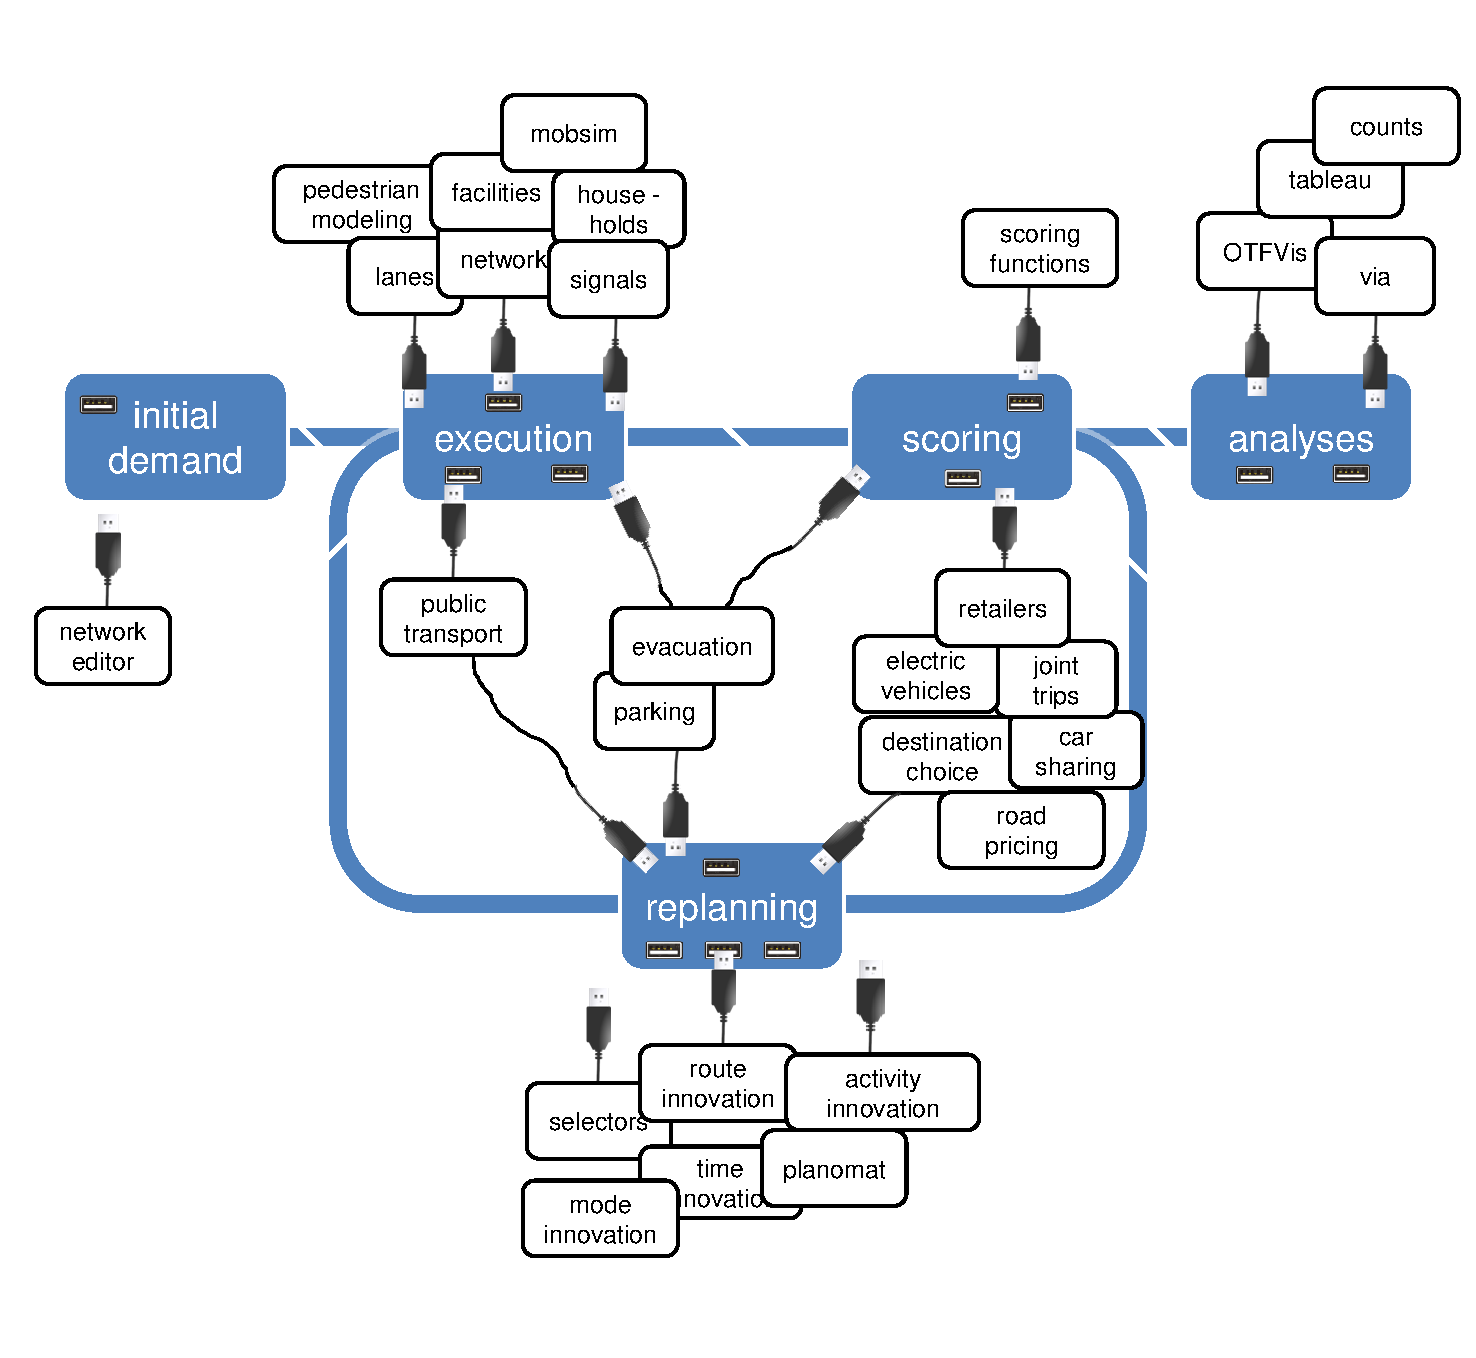
\includegraphics[width=0.99\textwidth, angle=0]{extending/figures/modules.pdf}}%
{}
The description of the modules in this and the following chapters is based on the categorization shown in Table~\ref{tab:modules}.
%
%\kai{TODO: macros for section names to re-use for table entries}
%\ah{Mache das später. Denke die jetzige Korrektur hält eine Weile}

\begin{center}
\begin{longtable}{|l|l|l|}
\caption{MATSim functionality overview}
\label{tab:modules} 
%\hline
%\textbf{Module} & \textbf{Type} &  \textbf{Described in} \\
%\hline
\endfirsthead
\hline
\multicolumn{3}{c}%
{\tablename\ \thetable\ -- \textit{Continued from previous page}} \\
\hline
%\textbf{Module} & \textbf{Type} &  \textbf{Described in} \\
%\hline
\endhead
\hline 
\multicolumn{3}{r}{\textit{Continued on next page}} \\
\endfoot
\hline
\endlastfoot
	\hline
	\textbf{MATSim Data Containers} & & Section~\ref{sec:using-data-containers} and \ref{sec:extending-data-containers} \\
	\hline
	Scenario & Core & Section~\ref{sec:extending-scenario} \\
	Network  & Core & Section~\ref{sec:using-network} and \ref{sec:extending-network} \\
	Population & Core & Section~\ref{sec:using-population} and \ref{sec:extending-population} \\
	Counts  & Main Distribution & Section~\ref{sec:extending-counts} \\
	Facilities & Main Distribution & Section~\ref{sec:extending-facilities} \\
	Households & Main Distribution & Section~\ref{sec:extending-households} \\
	Vehicles & Main Distribution & Section~\ref{sec:extending-vehicles} \\
	\hline
	\textbf{Global Modules and Global Aspects} & & Section~\ref{sec:using-globalmodules} and \ref{sec:extending-globalmodules} \\
	\hline
	Controler & Core & Section~\ref{sec:using-controler} and \ref{sec:extending-controler} \\
	Events & Core & Section~\ref{sec:using-events} \\
	Parallel Computing & Core & Section~\ref{sec:using-paralleleventhandling} \\
	Global & Core & Section~\ref{sec:using-global} \\
	\hline
	\textbf{Mobsims} & & Section~\ref{sec:using-mobsims} and \ref{sec:extending-mobsims} \\
	\hline
	QSim & Core & Section~\ref{sec:using-qsim} and \ref{sec:extending-qsim} \\
	JDEQSim & Core & Section~\ref{sec:using-jdeqsim} \\
	\hline
	\textbf{Scoring} & Core & Section~\ref{sec:using-scoring} \\
	\hline
	\textbf{Strategy Modules} & & Section~\ref{sec:strategymodules} \\
	\hline
	Time Innovation & Core & Section~\ref{sec:timechoice} \\
	Route Innovation & Core & Section~\ref{sec:routechoice} \\
	Mode Innovation & Core & Section~\ref{sec:modechoice} \\
	Selectors & Core & Section~\ref{sec:selectors} \\
	Destination Innovation & Contrib & Chapter~\ref{ch:destinationchoice} \\
	\hline
	\textbf{Observational Modules} & & Section~\ref{sec:observational} \\
	\hline
	Travel Time Calculator & Main Distribution & Section~\ref{sec:ttc} \\
	Link Stats & Main Distribution & Section~\ref{sec:linkStats} \\
	\hline
	\textbf{Further Modules} & &\\
	\hline
	Within-day Replanning & Main Distribution & Chapter~\ref{ch:withinday} \\
	Public Transport & Main Distribution/Contrib & Chapter~\ref{ch:pt} \\
	Multi-Modal Contribution & Contrib & Chapter~\ref{ch:multimodalsim} \\ % \ah{GTFS2TransitSchedule steckt da drin}
	Freight Traffic & Contrib & Chapter~\ref{ch:freight} \\
	Car Sharing & Playground & Chapter~\ref{ch:carsharing} \\
	Joint Trips and Social Networks & Playground & Chapter~\ref{ch:jointtrips} \\
	Dynamic Transport Systems & Contrib & Chapter~\ref{ch:dts} \\
	Parking & Contrib & Chapter~\ref{ch:parking} \\
	Electric Vehicles & Contrib & Chapter~\ref{ch:elvehicles} \\
	Air and Rail Transport & (see PT) & Chapter~\ref{ch:air} \\
	Roadpricing & Contrib & Chapter~\ref{ch:roadpricing} \\
	Emissions & Contrib & Chapter~\ref{ch:emissions} \\
	Accessibility & Contrib & Chapter~\ref{ch:accessibility} \\
	Evacuation & Contrib & Chapter~\ref{ch:evacuation}  \\
	Signals and Lanes & Main Distribution & Chapter~\ref{ch:signalslanes} \\
	PSim & Playground & Chapter~\ref{ch:psim} \\
	Cadyts & Contrib & Chapter~\ref{ch:cadyts} \\
	wagonSim & Contrib & Chapter~\ref{ch:wagonSim} \\
	\hline
	\textbf{Standalone Tools} & &\\ % Out-Of-The-Loop Tools
	\hline
	\gls{senozon} \gls{via} Visualizer & External & Chapter~\ref{ch:via} \\
	\gls{otfvis} Visualizer & Contrib & Chapter~\ref{ch:otfvis} \\	
	\gls{matsim}4UrbanSim & Contrib & Section~\ref{sec:matsim4urbansim} \\	
	Network Editors & External &  Chapter~\ref{ch:networkeditor} \\
	Interactive Analysis and Decision Support & External & Chapter~\ref{ch:businessanalytics} \\
\end{longtable}
\end{center}

%\kai{Andreas, m.E.\ ist der josm plugin von MZ und NK extern.  Könntest Du bitte (1) die beiden mal fragen, und (2) das entsprechend eintragen (hier und unter \url{matsim.org/extensions})?  Normalerweise würde ich das selber machen, würde das aber erst nach dem Urlaub schaffen.} 
%
%\ah{Hattest Recht, sind beide external (Berlin + Singapur). Die (old?) Contrib haben wir gar nicht im Buch}

% ##################################################################################################################
\section{MATSim Data Containers}
\label{sec:extending-data-containers}
%% \subsection{Supply-Side Data Containers}
%% \label{sec:supplysidemodules}
% ======================================================
\subsection{Scenario}
\label{sec:extending-scenario}

The \lstinline|scenario| module is
%, on the one hand, 
a container containing the main components of a scenario such as the \lstinline|config|, the \lstinline|network|, the \lstinline|population|, the \lstinline|facilities|, 
%the \lstinline|transitSchedule| \kai{unclear}, 
\lstinline|households| and \lstinline|vehicles|.

From a configuration perspective, the containers are available when a filename is given, otherwise not.  If an invalid filename is given, the code aborts with an error message.  If the code is configured in a way that it needs a container that was not loaded, it also aborts with an error message.

There are also switches of type \protect\lstinline|<param name="useHouseholds" value="..."/>| in the \lstinline|scenario| module of the config file.  These are deprecated and will eventually go away.  Until then, it may be that they have to be set correctly for the code to function. \chkAtEnd

From a programming perspective, arbitrary additional containers can be plugged into the global \lstinline|scenario| container.  See Section \ref{sec:scenario-extension-point} for more details.

%% \begin{itemize}\styleItemize
%% \item Invoking the module: (1) if you use Controler, scenario is always there. (2) otherwise, it needs to be generated explicitly in java.  \kai{chk}
%% \kai{Wir sind uns nicht im klaren darüber, was diese switches genau bedeuten, siehe \url{https://matsim.atlassian.net/browse/MATSIM-320}.  $\to$ weglassen.}

%% \item Configuration: There is a \lstinline|scenario| config file section, but we don't know what it means. \kai{chk} \ah{Hier haben wir doch eine kleine Inkonsistenz zwischen Container und Configuration Section. Config section definiert lanes, signals, households, vehicles, transit. Scenario hat aber z.B. facilities und population drin. Man sollte diese config section evtl. umbenennen in sowas wie optional\_scenario\_elements oder ähnlich. \url{https://matsim.atlassian.net/browse/MATSIM-320}}
%% \end{itemize}

%% The config file section is, on the other hand, used in a slightly different manner. It defines the usage of lanes, signal systems, road pricing, agent knowledges, vehicles, households and public transport. Still a respective config file section is required for every additional functionality. \kai{Ist das genau so?  Ich habe da ehrlich gesagt das genaue Design nie verstanden.  Oft für ein Eintrag in der scenario config group nur dafür, dass die Daten gelesen werden, und sonst passiert gar nichts.  Hm ...  Geradeziehen???}

% Code: \lstinline|org.matsim.core.scenario|

% ===================================================================================
\subsection{Network}
\label{sec:extending-network}
An important feature of the network module is using time-dependent network attributes. Network state changes can thus be considered, as \eg implied by accidents, and adaptive traffic control, with varying speed limits or driving directions of lanes on multi-lane roads with heavily unbalanced load over the course of a day. Attributes that can be adapted are ``free speed'', ``number of lanes'' and ``flow capacity''.

The adaptation can be specified by adding following two lines to the \lstinline|network| \gls{configfile} section:
\begin{xml}
<param name="timeVariantNetwork" value="true" />
<param name="inputChangeEventsFile" value="path_to_change_events_file" />
\end{xml}
%
An example snippet setting the free speed of three network links to zero approximately looks as follows:
%
%% <?xml version="1.0" encoding="UTF-8"?>
%% 	<networkChangeEvents xmlns="http://www.matsim.org/files/dtd"
%% 	xmlns:xsi="http://www.w3.org/2001/XMLSchema-instance"
%% 	xsi:schemaLocation="http://www.matsim.org/files/dtd
%% 	http://www.matsim.org/files/dtd/networkChangeEvents.xsd">}
\begin{xml}
  <networkChangeEvent startTime="03:06:00">
    <link refId="12487"/>
    <link refId="12489"/>
    <link refId="12491"/>
    <freespeed type="absolute" value="0.0"/>
  </networkChangeEvent>
\end{xml}
%% </networkChangeEvents>
%
\kai{add reference to real file}
\ah{no suitable one found :(}
\kai{Wir sollten eines nach examples/equil-extended einstellen.}

Alternatively, network change events can be directly added to the code using the method \lstinline|createNetworkChangeEvent| in class \lstinline|NetworkFactoryImpl|. An example can be found under \lstinline|org.matsim.integration.timevariantnetworks.QSimIntegrationTest| class.

\kai{Write RunXxx example!}

 %\ah{unfortunately no javadoc}
%
%\begin{lstlisting}
%networkChangeEvent =
	%network.getFactory().createNetworkChangeEvent(...);
%networkChangeEvent.setFlowCapacityChange(new ChangeValue(...));
%networkChangeEvent.setFreespeedChange(new ChangeValue(...));
%networkChangeEvent0.setLanesChange(new ChangeValue(...));
%network.addNetworkChangeEvent(networkChangeEvent);
%\end{lstlisting}
%
%\kai{lieber ein Verweis auf ein code snippet?  U.a. muss man auf NetworkImpl casten, was wir gerne irgendwann loswerden wollen und daher nicht im Buch haben wollen.}

% Code: \lstinline|org.matsim.core.network|

% ===================================================================================
\subsection{Population}
\label{sec:extending-population}
An powerful extension of a standard population can be achieved by specifying further agent attributes in a \lstinline|ObjectAttributes| file input to \gls{matsim} by parameter \lstinline|inputPersonAttributesFile|. Furthermore, subpopulations can be defined by parameter \lstinline|subpopulation|.

% Code: \lstinline|org.matsim.core.population|

% ===================================================================================
\subsection{Counts: \lstinline|counts.xml|}
\label{sec:extending-counts}
By providing a counts input file and configuring the \lstinline|counts| \gls{configfile} section \gls{matsim} plots link volume comparisons between hourly simulated and counted values for motorized individual traffic \citep{Horni_unpub_IVT_2007}. 

Simulating sample populations requires to scale the simulated volumes by the \lstinline|countsScaleFactor| parameter, \eg for a 10\,\% population this parameter needs to be set to~10.

\paragraph{Input:}
The following listing shows an example of a \lstinline|counts.xml| input file required to do traffic count comparisons. 

\begin{xml}
<?xml version="1.0" encoding="UTF-8"?> 
<counts name="example" desc="example counting stations" year="2015"> 
   <count loc_id="2" cs_id="005"> 
      <volume h="1" val="10.0"></volume> 
      <volume h="2" val="1.0"></volume> 
      <volume h="3" val="2.0"></volume> 
      <volume h="4" val="3.0"></volume> 
      <volume h="5" val="4.0"></volume> 
      <volume h="6" val="5.0"></volume> 
      <volume h="7" val="6.0"></volume> 
      <volume h="8" val="7.0"></volume> 
      <volume h="9" val="8.0"></volume> 
      <volume h="10" val="9.0"></volume> 
      <volume h="11" val="10.0"></volume> 
      <volume h="12" val="11.0"></volume> 
      <volume h="13" val="12.0"></volume> 
      <volume h="14" val="13.0"></volume> 
      <volume h="15" val="14.0"></volume> 
      <volume h="16" val="15.0"></volume> 
      <volume h="17" val="16.0"></volume> 
      <volume h="18" val="17.0"></volume> 
      <volume h="19" val="18.0"></volume> 
      <volume h="20" val="19.0"></volume> 
      <volume h="21" val="20.0"></volume> 
      <volume h="22" val="21.0"></volume> 
      <volume h="23" val="22.0"></volume> 
      <volume h="24" val="23.0"></volume> 
   </count> 
</counts>
\end{xml}
For a working example, check the \lstinline{examples/equil} directory in the \gls{matsim} directory tree (\cf Section~\ref{sec:settingUpMatsim}).

It starts with a header containing general descriptive information about the counts, including a year to describe how current the data is. Next, for each link having real world counts data, the hourly volumes can be specified. The network-link is referenced by the \lstinline|loc_id| attribute, in the example, it is link~2. The attribute \lstinline|cs_id| (counting station identifier) can be used to store an arbitrary description of the counting station. Most often it is used to note the original real word counting station to simplify future data comparison. The hourly volumes, specified by the hour of the day and its value, are optional: That is, not for every hour a value must be given. If for a counting station data is only available for certain hours of the day (\eg only during peak hours) it is possible to omit the other hours from the \gls{xml} listing. Note that the first hour of the day, from 0:00\,am to 1:00\,am, is numbered as ``1'', and \emph{not} by ``0'' as is often done in computer science.

\paragraph{Output:}
The counts module prints overview summaries for the whole network but also analyses for individual links, \ie a google maps based visualization is available, showing each station with a its load curve (see the example in Figure~\ref{fig:countcomparison}) in a pop-up window at the geographic location shown .

% ----------
\createfigure%
{Example for a link volumes comparison between simulation and road count values}%
{Example for a link volumes comparison between simulation and road count values}%
{\label{fig:countcomparison}}%
{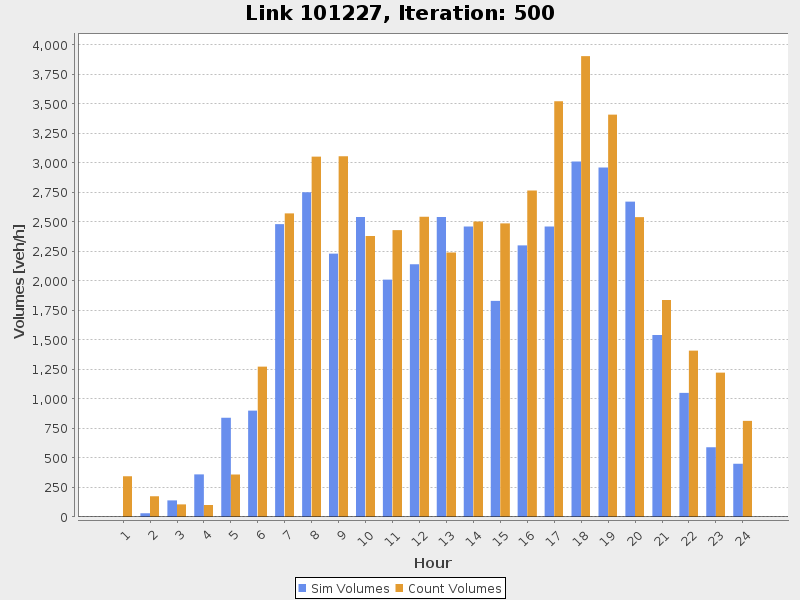
\includegraphics[width=0.7\textwidth, angle=0]{extending/figures/link101227.png}}%
{}
% ----------

%Public transport passenger counts are described in Chapter~\ref{ch:pt}. \ah{check} \ah{nothing there}

As shown by \citet[][]{BalmerEtAl_ResRep_bdktzrh_2009}, for the Zürich scenario link volume comparisons have been successfully performed with data based on city level, cantonal level and national level \citep[][]{ASTRA_Webpage_2006}, where an average working day (Monday to Thursday, excluding public holidays) was built. Usually it is helpful to exclude a substantial part of the outer range of the modeled study region to prevent boundary effects.

% Code: \lstinline|org.matsim.counts|

% ===================================================================================
\subsection{Facilities}
\label{sec:extending-facilities}
Facilities are an optional element of \gls{matsim}, some \glspl{module}, such as the destination innovation module (Chapter~\ref{ch:destinationchoice}), use it, however.
If \gls{matsim} \glspl{facility} are used, the agents perform their activities in a specific \gls{facility} attached to a network link. 

Facilities are included in the scenario by defining the \lstinline|facilities| \gls{configfile} section and providing a facilities file, approximately looking as follows.
%
\begin{xml}
...
<facilities name="test facilities for triangle network">
	<facility id="1" x="60.0" y="110.0">
		<activity type="home" />
	</facility>
	<facility id="10" x="110.0" y="270.0">
		<activity type="education" />
	</facility>
</facilities>
\end{xml}
%
Besides activities, that can be done in the facility, further location attributes, such as open times, can be specified. 
A working example facilities file can be found in the \gls{matsim} directory tree in the \lstinline{examples/siouxfalls-2014} directory.

Facilities are mostly used in the \gls{matsim} Zürich group, in particular in the Zürich scenario, where facilities are derived from the Federal Enterprise Census~2001 \citep[][]{SwissEnterpriseCensus_manual_2001} providing hectare level information and using NOGA-classification. Detailed technical description of facilities generation is given by \citet[][]{Meister_TechRep_IVT_2008, Meister_unpub_IVT_2007}. Comparable data is available in most countries from official sources, such as censuses, and commercial sources, such as navigation network providers, yellow pages publishers or business directories, and last but not least google and \gls{osm} \citep[][]{OpenStreetMap_Webpage_2015}.

% Code:\lstinline|org.matsim.core.facilities|

% ##################################################################################################################
%% \subsection{Demand-Side Data Containers}
%% \label{sec:dsm}

% ===================================================================================
\subsection{Households}
\label{sec:extending-households}
Households are another optional element of \gls{matsim}. To load households into a scenario, the \lstinline|useHouseholds| parameter in the \lstinline|scenario| \gls{configfile} section must be set to true. Furthermore the \gls{configfile} must contain a section \lstinline|households|. This section should specify the paths to a file containing households (parameter \lstinline|inputFile|) and a file containing further household attributes (parameter \lstinline|inputHouseholdAttributesFile|).

% \ah{households file listing?} \ah{maybe next revision}

% Code: \lstinline|org.matsim.households|

% ===================================================================================
%% \subsection{Data containers belonging both to demand and to supply}
\subsection{Vehicles}
\label{sec:extending-vehicles}
Vehicles are an optional element of \gls{matsim}. To load vehicles into a scenario, the \lstinline|useVehicles| parameter in the \lstinline|scenario| \gls{configfile} section must be set to true. Furthermore the \gls{configfile} must contain a section \lstinline|vehicles|. This section should specify the paths to a file containing vehicles (parameter \lstinline|vehiclesFile|). 

\ah{Amit: ``At the moment, different vehicleTypes and vehicles are not added using 'VehiclesFile' instead they are added to scenario directly.''

ah.chk. I guess this now has changed with Kai's refactoring? Or does it still need to be ``scripted''?
}

Furthermore, there exists the possibility to use \lstinline|VehicleUtils| for specifying mode vehicles according to the example syntax in \lstinline{RunMobsimWithMultipleModeVehiclesExample} under \url{http://matsim.org/javadoc} $\to$ core (see also Section~\ref{sec:using-qsim-multimodal}). 

%\citet[][]{JaeggiEtAl_TRR_2012} might serve as an empirical base for the assignment of vehicles to agents or households. \ah{Füllsatz}

%\kai{Andreas, habe jetzt die transitXxx file formats in das pt chapter verschoben.  Meine Intuition ist zwar eigentlich, dass sie besser ``Infrastruktur'' (als ``shared'') Container wären.  Aber Marcel hat das bis jetzt anders gesagt, und es ist auch kein so großes Problem.} \kai{Siehe auch \url{https://matsim.atlassian.net/browse/MATSIM-332}.} \ah{ok}

%\kai{Folgendes muss noch geschrieben werden.} \ah{done}

%% \kai{Bin mir ziemlich sicher, dass wir hier nur die ``vehicles'' lassen sollten, und die ``transitVehicles'' erst mit der entsprechenden extension erklären sollten.  Auch die freightVehicles sind schließlich nicht global verfügbar, sondern nur im Rahmen der extension.}

%% \kai{Folgendes ist nicht operational.  Sehe im Moment gar nicht, wie wir das Buch sinnvoll fertig schreiben können, ohne das gelöst zu haben, aber ich sehe auch nicht, wo die Zeit herkommen soll.}
%% %
%% \kai{Ok, in einem Anfall von Verzweiflung habe ich das gestern eingebaut: vehicles und transitVehicles sind nun separat.  Allerdings laufen die automatischen Tests im Moment irgendwie nicht; das sollte man vielleicht noch abwarten.}

%% \kai{Von der Logik her sollen die ``useXxx'' switches im scenario module der config auch noch weg.  Aber im Moment geht das nicht ohne größeren Umstand.}

%% A private household's decision to buy a vehicle in order to satisfy one's transport needs is a demand side decision.
%% %
%% However, if a public transit company decides to buy buses of a certain type, this is more a supply side decision (to supply potential passengers with a vehicle) than a demand side decision (the vehicle will have a demand for road space once it runs).

%% \begin{itemize}\styleItemize
%% \item Invoking the module: Vehicles need to be enabled in the \lstinline|scenario| configuration file section.
%% \item Configuration: At the moment vehicles are only used for public transport (Chapter~\ref{ch:pt}), \ie motorized individual traffic vehicles are not used in \gls{matsim} nowadays. Thus, the configuration file section specifying the input file is located in the \lstinline|transit| configuration file section, while the vehicles module does not have its own configuration file section. 
%% \ah{Klären, ob man diese kleine Inkonsistenz beheben möchte.}  
%% \kai{Ist das nicht schon erledigt?}
%% \ah{final String vehiclesFile = this.config.transit().getVehiclesFile();}
%% \kai{Arghh.}
%% \ah{\url{https://matsim.atlassian.net/browse/MATSIM-314}}
%% %
%% This might change one day when the parking module will start to use vehicles. 
%% \end{itemize}

%% The vehicles package provides a file reader and a factory to create vehicles.

% Code: \lstinline|org.matsim.vehicles|


%##################################################################################################################
\section{Global Modules and Global Aspects}
\label{sec:extending-globalmodules}
% ===================================================================================
\subsection{Controler}
\label{sec:extending-controler}
The controler module, can be extended by \lstinline|Events| and \lstinline|Listeners| as detailed in Chapter~\ref{ch:extensionpoints}. 
%% Classes implementing one or more \lstinline|Listener Interfaces| and can be registered with the Controler with \lstinline|addControlerListener()|. The controler fires \lstinline|Controler Events| at specific points during the run to the registered \lstinline|Listeners|, which can then execute their own code.
%
%Das ist nur ein Ausschnitt von dem, was der Controler kann.  Da es im entsprechenden Kap. ja beschrieben wird, brauchen wir das hier m.E. nicht nochmal. kai, dec'14

%% \textcolor{gray}{\st{Another possibility to customize the controler is by inheritence from the class} \lstinline|org.matsim.core.controler|.}  \kai{Please do not do or advertise this any more.}

% ##################################################################################################################
\section{Mobility Simulations}
\label{sec:extending-mobsims}
% ===================================================================================
\subsection{\protect\gls{qsim}}
\label{sec:extending-qsim}
The simulation is able to handle time-variant networks, within-day replanning \citep[][]{Dobler_TechRep_IVT_2009}, and in an experimental manner traffic lights \citep[][]{Neumann_MastersThesis_2008}).

Section~\ref{sec:using-othermodesthancar} details the necessary steps to simulate a multi-modal scenario; Section~\ref{sec:using-qsim-multimodal} therein focuses on \gls{qsim}. 
In addition to that, arbitrary vehicles can be included as follows. 
Assigning vehicles of a specific type to agents is done
\begin{itemize}\styleItemize 
\item by specifying a vehicles input file \protect\lstinline|<param name="vehiclesFile" value="..." />|, or
\item by creating mode vehicles as shown above. 
\end{itemize}
%\kai{Das stimmt so nicht.  Man kann \emph{entweder} die vehicles Datei verwenden.  \emph{Oder} man definiert die mode vehicles.  Revise.} \ah{danke}

Simulation experiments for \gls{qsim}'s relatively new \gls{multimodal} feature, applying multiple mode vehicles, have been performed for the Patna scenario as reported in Chapter~\ref{ch:patna}.

An earlier \gls{multimodal} approach targeted at overcoming the \gls{teleportation} estimates of non-motorized modes, particularly focused on pedestrians, is presented in Chapter~\ref{ch:multimodalsim}.

% --------------------------------------
%\subsubsection{Multi-Modal Simulation With QSim}
%\label{sec:multimodalsim_qsim}
%\gls{qsim} can simulate \gls{multimodal} traffic. Congested modes, \ie modes simulated not only \gls{teleported}, are specified by the parameter \lstinline|mainMode|. Technically, these are the modes that the departure handler of the \lstinline|netsimengine| handles 
%\footnote{Effective cell size, effective lane width, flow capacity factor, and storage capacity factor need to be set with diligence.}. 
%Theoretically also pedestrians can be included, however, only vehicular modes actually make sense, \ie car, bike, and public transport, in particular buses.
 
%\ah{Is that true with pt? Do we actually have all the vehicular traffic interactions in \gls{qsim}?}. 
%Assigning vehicles of a specific type to agents is done with in the vehicles input file \lstinline|<param name="vehiclesFile" value="..." />|. 
%\ah{is that the only place necessary?}. 
%Further configuration necessary to include public transport is detailed in Chapter~\ref{ch:pt}.

%To model mode interactions, a fully \gls{multimodal} network, \ie a network that has links being shared by different modes must be provided. 
%As shown in Section~\ref{sec:lgstarted-network-file}, specification of link modes is done with the network attribute \lstinline|modes|.
%Furthermore, the router needs to be informed about the network modes by the \lstinline|planscalcroute| parameter \lstinline|<param name="networkModes" value="car,ride" />|.
%\ah{is this a double configuration, qsim and planscalcroute? can we merge them?}

%The mode interactions can be further specified by \gls{qsim} parameter \lstinline|linkDynamics|. 
%This parameter is also productive for car mode only, but it is particularly important for multi-modal scenarios. 
%Dynamics either follow strict \gls{fifo} or include passing, \ie \lstinline$<param name="linkDynamics" value="FIFO|PassingQ" />$. 

%Simulation experiments for \gls{qsim}'s relatively new \gls{multimodal} feature, applying multiple mode vehicles, have been performed for the Patna scenario as reported in Chapter~\ref{ch:patna}.

%An earlier \gls{multimodal} approach targeted at overcoming the \gls{teleportation} estimates of non-motorized modes, particularly focused on pedestrians, is presented in Chapter~\ref{ch:multimodalsim}.

%\ah{Amit, Kai: Please check this section. Thanks.}

% ##################################################################################################################
% Local Variables:
% mode: latex
% mode: reftex
% mode: visual-line
% TeX-master: "../../main"
% comment-padding: 1
% fill-column: 9999
% End: 
